\documentclass{beamer}
% Theme Matrix: http://www.hartwork.org/beamer-theme-matrix/
\mode<presentation> { \usetheme{Malmoe}\usecolortheme{dove} }
\setbeamertemplate{itemize items}[default]
\usepackage[T1]{fontenc}
\usepackage{parskip,graphics,tikz,multimedia,hyperref,ulem,multicol}
\usetikzlibrary{arrows,positioning,shapes,decorations.pathmorphing,snakes}
\setlength{\itemsep}{0pt}\setlength{\parskip}{0pt}\setlength{\parsep}{0pt}
\graphicspath{{./images/}}

\usepackage{listings,textcomp,color}
\lstset{language=Python,upquote=true,
  basicstyle=\ttfamily\tiny,numbers=left,
  numberstyle=\tiny,stepnumber=1,numbersep=5pt,
  backgroundcolor=\color{white},frame=single,tabsize=2,
  showspaces=false,showstringspaces=false,showtabs=false,
  breaklines=true,breakatwhitespace=true,escapeinside={\%*}{*)},
  keywordstyle=\color{blue!70},stringstyle=\color{green!70!black!70},
  commentstyle=\color{black!80}\it
}
\lstdefinelanguage{scala}{
  morekeywords={abstract,case,catch,class,def,%
    do,else,extends,false,final,finally,%
    for,if,implicit,import,match,mixin,%
    new,null,object,override,package,%
    private,protected,requires,return,sealed,%
    super,this,throw,trait,true,try,%
    type,val,var,while,with,yield},
  otherkeywords={=>,<-,<\%,<:,>:,\#,@},
  sensitive=true,
  morecomment=[l]{//},
  morecomment=[n]{/*}{*/},
  morestring=[b]",
  morestring=[b]',
  morestring=[b]"""
}

\usebackgroundtemplate{
  \tikz[overlay,remember picture]
  \node[yshift=10mm,anchor=south east,inner sep=0pt]
    at (current page.south east) {
    % Add small logo here if desired.
    % \includegraphics[width=0.5in]{logo.png}
  };
}

\tikzset{
  yn/.style={draw,thick,rounded corners,fill=yellow!20,inner sep=.3cm},
  bn/.style={draw,thick,rounded corners,fill=blue!05,inner sep=.3cm},
  on/.style={draw,thick,rounded corners,fill=orange!20,inner sep=.3cm},
  rn/.style={draw,thick,rounded corners,fill=red!20,inner sep=.3cm},
  greenn/.style={draw,thick,rounded corners,fill=green!20,inner sep=.3cm},
  grayn/.style={draw,thick,rounded corners,fill=gray!20,inner sep=.3cm},
  to/.style={
    ->,>=stealth',shorten >=1pt,semithick,font=\sffamily\footnotesize
  },
  from/.style={
    <-,>=stealth',shorten >=1pt,semithick,font=\sffamily\footnotesize
  },
  tofrom/.style={
    <->,>=stealth',shorten >=1pt,semithick,font=\sffamily\footnotesize
  },
  every node/.style={align=center},
  squig/.style={->,line join=round,decorate, decoration={zigzag,
    segment length=8,amplitude=2,post=lineto,post length=2pt}}
}

\newcommand{\uncheckedBox}{\ensuremath{\square}}
\newcommand{\checkedBox}{\ensuremath{\text{\rlap{\checkmark}}\square}}

\expandafter\def\expandafter\insertshorttitle\expandafter{%
  \insertshorttitle\hfill%
  \insertframenumber\,/\,\inserttotalframenumber}

\begin{document}
\title{Beamer Snippets}\author{Brandon Amos}\date{July 2014}

\section{Section 1}
\subsection{Subsection A}
% Reference: http://stackoverflow.com/questions/217834
\frame{\frametitle{\insertsection}\framesubtitle{\insertsubsection}
  \begin{center}
   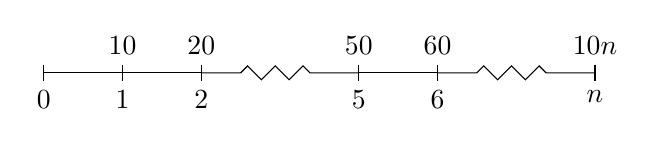
\begin{tikzpicture}[
      snake=zigzag,line before snake=5mm,line after snake=5mm
    ]
    \draw (0,0) -- (2,0);
    \draw[snake] (2,0) -- (4,0);
    \draw (4,0) -- (5,0);
    \draw[snake] (5,0) -- (7,0);

    \foreach \x in {0,1,2,4,5,7} \draw (\x cm,3pt) -- (\x cm,-3pt);

     \draw (0,0) node[below=3pt] {$ 0 $} node[above=3pt] {$   $};
     \draw (1,0) node[below=3pt] {$ 1 $} node[above=3pt] {$ 10 $};
     \draw (2,0) node[below=3pt] {$ 2 $} node[above=3pt] {$ 20 $};
     \draw (3,0) node[below=3pt] {$  $} node[above=3pt] {$  $};
     \draw (4,0) node[below=3pt] {$ 5 $} node[above=3pt] {$ 50 $};
     \draw (5,0) node[below=3pt] {$ 6 $} node[above=3pt] {$ 60 $};
     \draw (6,0) node[below=3pt] {$  $} node[above=3pt] {$  $};
     \draw (7,0) node[below=3pt] {$ n $} node[above=3pt] {$ 10n $};
    \end{tikzpicture}
  \end{center}
}

\end{document}